\documentclass[onesided]{article}\usepackage[]{graphicx}\usepackage[]{color}
% maxwidth is the original width if it is less than linewidth
% otherwise use linewidth (to make sure the graphics do not exceed the margin)
\makeatletter
\def\maxwidth{ %
  \ifdim\Gin@nat@width>\linewidth
    \linewidth
  \else
    \Gin@nat@width
  \fi
}
\makeatother

\definecolor{fgcolor}{rgb}{0.345, 0.345, 0.345}
\newcommand{\hlnum}[1]{\textcolor[rgb]{0.686,0.059,0.569}{#1}}%
\newcommand{\hlstr}[1]{\textcolor[rgb]{0.192,0.494,0.8}{#1}}%
\newcommand{\hlcom}[1]{\textcolor[rgb]{0.678,0.584,0.686}{\textit{#1}}}%
\newcommand{\hlopt}[1]{\textcolor[rgb]{0,0,0}{#1}}%
\newcommand{\hlstd}[1]{\textcolor[rgb]{0.345,0.345,0.345}{#1}}%
\newcommand{\hlkwa}[1]{\textcolor[rgb]{0.161,0.373,0.58}{\textbf{#1}}}%
\newcommand{\hlkwb}[1]{\textcolor[rgb]{0.69,0.353,0.396}{#1}}%
\newcommand{\hlkwc}[1]{\textcolor[rgb]{0.333,0.667,0.333}{#1}}%
\newcommand{\hlkwd}[1]{\textcolor[rgb]{0.737,0.353,0.396}{\textbf{#1}}}%
\let\hlipl\hlkwb

\usepackage{framed}
\makeatletter
\newenvironment{kframe}{%
 \def\at@end@of@kframe{}%
 \ifinner\ifhmode%
  \def\at@end@of@kframe{\end{minipage}}%
  \begin{minipage}{\columnwidth}%
 \fi\fi%
 \def\FrameCommand##1{\hskip\@totalleftmargin \hskip-\fboxsep
 \colorbox{shadecolor}{##1}\hskip-\fboxsep
     % There is no \\@totalrightmargin, so:
     \hskip-\linewidth \hskip-\@totalleftmargin \hskip\columnwidth}%
 \MakeFramed {\advance\hsize-\width
   \@totalleftmargin\z@ \linewidth\hsize
   \@setminipage}}%
 {\par\unskip\endMakeFramed%
 \at@end@of@kframe}
\makeatother

\definecolor{shadecolor}{rgb}{.97, .97, .97}
\definecolor{messagecolor}{rgb}{0, 0, 0}
\definecolor{warningcolor}{rgb}{1, 0, 1}
\definecolor{errorcolor}{rgb}{1, 0, 0}
\newenvironment{knitrout}{}{} % an empty environment to be redefined in TeX

\usepackage{alltt}
\usepackage[T1]{fontenc}
\linespread{1.5} % Line spacing - Palatino needs more space between lines
\usepackage{microtype} % Slightly tweak font spacing for aesthetics

\usepackage[hmarginratio=1:1,columnsep=20pt]{geometry} % Document margins
%\usepackage{multicol} % Used for the two-column layout of the document
\usepackage[hang, small,labelfont=bf,up,textfont=it,up]{caption} % Custom captions under/above floats in tables or figures
\usepackage{booktabs} % Horizontal rules in tables
\usepackage{float} % Required for tables and figures in the multi-column environment - they need to be placed in specific locations with the [H] (e.g. \begin{table}[H])

\usepackage{lettrine} % The lettrine is the first enlarged letter at the beginning of the text
\usepackage{paralist} % Used for the compactitem environment which makes bullet points with less space between them

% to ignore texts: good for thank messages and paper submissions.
      % \fbox{\phantom{This text will be invisible too, but a box will be printed arround it.}}

\usepackage{abstract} % Allows abstract customization
\renewcommand{\abstractnamefont}{\normalfont\bfseries} % Set the "Abstract" text to bold
%\renewcommand{\abstracttextfont}{\normalfont\small\itshape} % Set the abstract itself to small italic text

\usepackage[]{titlesec} % Allows customization of titles
\renewcommand\thesection{\Roman{section}} % Roman numerals for the sections
\renewcommand\thesubsection{\Roman{subsection}} % Roman numerals for subsections
\titleformat{\section}[block]{\large\scshape\centering}{\thesection.}{1em}{} % Change the look of the section titles
\titleformat{\subsection}[block]{\large}{\thesubsection.}{1em}{} % Change the look of the section titles

\usepackage{fancybox, fancyvrb, calc}
\usepackage[svgnames]{xcolor}
\usepackage{physics}
\usepackage{epigraph}
\usepackage{longtable}
\usepackage{pdflscape}
\usepackage{graphics}
\usepackage{pbox} % \pbox{20cm}{This is the first \\ cell}
\usepackage{amsfonts}
\usepackage{amsmath}
\usepackage{amssymb}
\usepackage{rotating}
\usepackage{paracol}
\usepackage{textcomp}
\usepackage[export]{adjustbox}
\usepackage{afterpage}
\usepackage{filecontents}
\usepackage{color}
\usepackage{latexsym}
\usepackage{lscape}       %\begin{landscape} and \end{landscape}
\usepackage{wasysym}
\usepackage{dashrule}
\usepackage{marvosym} % face package
\usepackage{framed}
\usepackage{tree-dvips}
\usepackage{pgffor}
\usepackage[]{authblk}
\usepackage{setspace}
\usepackage{array}
\usepackage[latin1]{inputenc}
\usepackage{hyperref}     %desactivar para link rojos
\usepackage{graphicx}
\usepackage{dcolumn} % for R tables
\usepackage{multirow} % For multirow in tables
\usepackage{pifont}
\usepackage{listings}
\usepackage{bm}




% hypothesis / theorem package begin
\usepackage{amsthm}
\usepackage{thmtools}
\declaretheoremstyle[
spaceabove=6pt, spacebelow=6pt,
headfont=\normalfont\bfseries,
notefont=\mdseries, notebraces={(}{)},
bodyfont=\normalfont,
postheadspace=0.6em,
headpunct=:
]{mystyle}
\declaretheorem[style=mystyle, name=Hypothesis, preheadhook={\renewcommand{\thehyp}{H\textsubscript{\arabic{hyp}}}}]{hyp}

\usepackage{cleveref}
\crefname{hyp}{hypothesis}{hypotheses}
\Crefname{hyp}{Hypothesis}{Hypotheses}
% hypothesis / theorem package end


%----------------------------------------------------------------------------------------
% Other ADDS-ON
%----------------------------------------------------------------------------------------

% independence symbol \independent
\newcommand\independent{\protect\mathpalette{\protect\independenT}{\perp}}
\def\independenT#1#2{\mathrel{\rlap{$#1#2$}\mkern2mu{#1#2}}}







\hypersetup{
    bookmarks=true,         % show bookmarks bar?
    unicode=false,          % non-Latin characters in Acrobat's bookmarks
    pdftoolbar=true,        % show Acrobat's toolbar?
    pdfmenubar=true,        % show Acrobat's menu?
    pdffitwindow=true,     % window fit to page when opened
    pdfstartview={FitH},    % fits the width of the page to the window
    pdftitle={My title},    % title
    pdfauthor={Author},     % author
    pdfsubject={Subject},   % subject of the document
    pdfcreator={Creator},   % creator of the document
    pdfproducer={Producer}, % producer of the document
    pdfkeywords={keyword1} {key2} {key3}, % list of keywords
    pdfnewwindow=true,      % links in new window
    colorlinks=true,       % false: boxed links; true: colored links
    linkcolor=ForestGreen,          % color of internal links (change box color with linkbordercolor)
    citecolor=ForestGreen,        % color of links to bibliography
    filecolor=ForestGreen,      % color of file links
    urlcolor=ForestGreen           % color of external links
}

%\usepackage[nodayofweek,level]{datetime} % to have date within text

\newcommand{\LETT}[3][]{\lettrine[lines=4,loversize=.2,#1]{\smash{#2}}{#3}} % letrine customization



% comments on margin
  % Select what to do with todonotes: 
  % \usepackage[disable]{todonotes} % notes not showed
  \usepackage[draft]{todonotes}   % notes showed
  % usage: \todo{This is a note at margin}

\usepackage{cooltooltips}

%%% bib begin
\usepackage[american]{babel}
\usepackage{csquotes}
\usepackage[backend=biber,style=authoryear,dashed=false,doi=false,isbn=false,url=false,arxiv=false]{biblatex}
%\DeclareLanguageMapping{american}{american-apa}
\addbibresource{/Users/hectorbahamonde/Bibliografia_PoliSci/library.bib} 
\addbibresource{/Users/hectorbahamonde/Bibliografia_PoliSci/Bahamonde_BibTex2013.bib} 

% USAGES
%% use \textcite to cite normal
%% \parencite to cite in parentheses
%% \footcite to cite in footnote
%% the default can be modified in autocite=FOO, footnote, for ex. 
%%% bib end

\usepackage{fancyhdr} % Headers and footers
\pagestyle{fancy} % All pages have headers and footers
\fancyhead{} % Blank out the default header
\fancyfoot{} % Blank out the default footer
\fancyhead[C]{MLE para Outcomes Poco Frecuentes: Zero-Inflated Poisson y Rare Event Logistic } % Custom header text
\fancyfoot[RO,LE]{\thepage} % Custom footer text
\IfFileExists{upquote.sty}{\usepackage{upquote}}{}
\begin{document}
% DOCUMENT ID
%----------------------------------------------------------------------------------------
%	CONTENT
%----------------------------------------------------------------------------------------

%\graphicspath{
%{/Users/hectorbahamonde/RU/Term5/Experiments_Redlawsk/Experiment/Data/}
%}



%%%%%%%%%%%%%%%%%%%%%%%%%%%%%%%%%%%%%%%%%%%%%%
% begin knitr stuff


%%%%%%%%%%%%%%%%%%%%%%%%%%%%%%%%%%%%%%%%%%%%%%





\hspace{-5mm}{\bf Profesor}: H\'ector Bahamonde, PhD.\\
\texttt{e:}\href{mailto:hector.bahamonde@uoh.cl}{\texttt{hector.bahamonde@uoh.cl}}\\
\texttt{w:}\href{http://www.hectorbahamonde.com}{\texttt{www.hectorbahamonde.com}}\\
{\bf Curso}: MLE.\\
\hspace{-5mm}{\bf TA}: Gonzalo Barr\'ia.

\section{Outcomes Poco Frecuentes}

En esta clase seguiremos con los \emph{outcomes} de ``cuentas''. En las ciencias sociales existen \emph{data generating processes} que son raros. Es decir, ocurren con poca frecuencia. Ejemplos son n\'umero de atentados terroristas, secuestros, etc. Ser\'ia muy raro que por ejemplo al d\'ia y de manera constante, existiera mas de cero secuestro. 

Aunque una opci\'on ser\'ia dejar de lado un estudio as\'i (porque ``\emph{qui\'en se interesar\'ia en estudiar algo que casi nunca pasa?}''), existen razones substantivas para estudiar fen\'omenos que ocurren rara vez. Que un evento ocurra rara vez no lo hace menos importante. Por ejemplo, atentados a autoridades ocurren rara vez, pero {\bf ser\'ia incorrecto pensar que el fen\'omeno carece de inter\'es}.

En la primera mitad de la clase abordaremos el modelo Zero-Inflated (con variantes Poisson/Negative-Binomial). En la segunda mitad del curso veremos una generalizaci\'on del modelo logit pero calibrado para dar cuenta a eventos raros. 

\subsection{Zero-Inflated}

\paragraph{Motivaci\'on} El modelo zero-inflated justamente da cuenta de fen\'omenos donde los casos donde el evento ocurre es casi en su gran mayor\'ia un ``0''. Es por esto que se llama ``zero-inflated'', i.e. la cantidad 0 est\'a ``inflada''.

La caracter\'istica principal de la regresi\'on zero-inflated es que modela dos procesos de manera separada. Por un lado, modela aquellos casos donde $y_{i}>0$, y aparte, modela aquellos casos donde $y_{i}=0$. 

\paragraph{Supuestos distribucionales} Los eventos que no son ceros se modelan seg\'un la distribuci\'on Poisson, donde


\begin{equation}\label{poisson:d}
Pr(y_{i}|\mu) = \frac{\text{exp}(-\mu)\mu^{y_{i}}}{y_{i}!}
\end{equation}

donde $\mu=\text{exp}(\boldsymbol{x}_{i}\boldsymbol{\beta})$. Si te fijas, hasta el momento, todo sigue igual al modelo Poisson. 

Donde el modelo Zero-inflated (Poisson) se diferencia del modelo Poisson (a secas) es que los casos donde $y_{i}=0$ son modelados de manera separada, donde $Pr(y_{i})=0=\psi$. Lo interesante, es que estas probabilidades $\psi$ son modeladas como funci\'on de las caracteristicas de los respondentes/firmas/ciudades, i.e. de la unidad de an\'alisis. M\'as formalmente,


\begin{equation}\label{psi:p}
\psi_{i} = F(\boldsymbol{x}_{i}\boldsymbol{\beta})
\end{equation}

donde $F$ es el \emph{cumulative density function} de la distribuci\'on normal ($\Phi$) o de la distribuci\'on logit ($\pi$), es decir $F=\{\Phi, \pi\}$. Si te fijas, el proceso que modela los 0's se gu\'ia por el mismo proceso que modelaba \emph{outcomes} binarios. En este caso, el proceso que modela los 0's modela casos donde hay ceros (1) o no (0).

Veamos en m\'as detalle c\'omo combinamos las probabilidades del modelo Poisson que modela los \emph{outcomes} $y_{i}>0$ y las probabilidades del modelo binario para \emph{outcomes} $y_{i}=0$,

\begin{equation}\label{zip:p}
\begin{split}
\text{Pr}(y_{i}=0|\boldsymbol{x}_{i}) &= \psi_{i}+(1-\psi_{i})\text{exp}(-\mu)\\
\text{Pr}(y_{i}|\boldsymbol{x}_{i}) &= (1-\psi_{i})\frac{\text{exp}(-\mu)\mu^{y_{i}}}{y_{i}!} \;\; \text{for} \; y_{i}>0
\end{split}
\end{equation}

\autoref{zip:p} es lo que llamamos el modelo Zero-inflated Poisson (``ZIP''). Como ya sabemos, el modelo Poisson descansa sobre el supuesto de la {\bf equidispersi\'on}. Este supuesto no siempre se cumple. Afortunadamente, existe una extensi\'on que (sorpresa!) se llama {\bf Zero-Inflated Negative Binomial} (``ZINB''). Aunque no entraremos en el detalle de la notaci\'on de los modelos ZINB, ya sabemos que se obtiene modificando la varianza y el valor esperado de cuentas $\mu$.

Sin embargo, lo que s\'i discutiremos es como ayudar a dilucidar qu\'e modelo hace un mejor trabajo maximizando el likelihood. Para esto usaremos el Vuong test que nos dice si el ``ZIP'' tiene un mejor \emph{fit} que el ``ZINB''.




\subsection{Rare-event Logistic}

\paragraph{Motivaci\'on} Los modelos generalizados son flexibles y existen muchas maneras posibles de abordar procesos que son similares. Tanto el ZIP como el ZINB parten de la base que el \emph{data generating process} genera outcomes poco frecuentes. Ambos modelan cuentas. Qu\'e pasa cuando no quieres estimar cuentas si no que un proceso binario (0,1) pero donde es muy raro encontrar 1's? Para estos casos existen modelos log\'isticos especiales llamados ``\emph{rare event logistic regressions}'' (\emph{relogit}).

\textcite{King2001} derivan el \emph{rare-event logistic regression}. Particularmente, ellos lo piensan para casos de guerra (1) o paz (0), donde la guerra es (afortunadamente) mucho menos frecuente que la paz \parencite{King2001a}.

\paragraph{Parametrizaci\'on} Recordemos el modelo logit tradicional que est\'a dado por,

\begin{equation}\label{logit:pr}
\text{Pr}(y_{i}=1)=\pi_{i}
\end{equation}


donde,


\begin{equation}\label{logit}
\pi_{i} = \frac{exp(\boldsymbol{x}_{i}^{\prime}\boldsymbol{\beta})}{1+exp(\boldsymbol{x}_{i}^{\prime}\boldsymbol{\beta})}
\end{equation}

Como explican \textcite[149]{King2001}, el modelo logit para eventos raros, est\'a caracterizado por un ``\emph{{\bf corrector factor}}'' $C_{i}$ que {\bf incrementa en 50\% la contribuci\'on relativa} de instancias donde $y_{i}=1$, i.e. haciendo ``menos raras'' estas realizaciones. El entendido es que un ``evento raro'' ocurre menos de la mitad de las veces. 

De manera muy similar a la regresi\'on logit en \autoref{logit:pr}, la probabilidad estimada del \emph{rare event logistic regression} est\'a dado por,

\begin{equation}\label{corrector:factor:1}
\text{Pr}(y_{i}=1)=\pi_{i} + C_{i}
\end{equation}

donde el \emph{corrector factor} est\'a caracterizado por,


\begin{equation}\label{corrector:factor:2}
C_{i} = (0.5-\pi_{i})\pi_{i}(1-\pi_{i})\boldsymbol{x}V(\boldsymbol{\beta})\boldsymbol{x}^{T}
\end{equation}

Como ellos explican, ``[w]hen $\pi_{i} < 0.5$, as is usually the case for rare events, the correction factor adds to the estimated probability of an event'' \parencite[149]{King2001}. Uno de los entendidos m\'as importantes de esta soluci\'on es que en {\bf finite samples} la incertidumbre relativa de los eventos del tipo $y_{i}=1$ es mayor e inconsistente. 

Esto se puede ver en la varianza de un modelo logit,

\begin{equation}\label{var:logit}
V(\boldsymbol{\beta}) = [\sum_{1}^{N}\pi_{i}(1-\pi_{i})\boldsymbol{x}_{i}^{T}\boldsymbol{x}_{i}]^{-1}
\end{equation}

donde ``[t]he part of this matrix affected by rare events is the factor $\pi_{i}(1-\pi_{i})$'' \parencite[141]{King2001}. Como ellos explican, en los estudios con eventos raros, el resultado es que ``$\pi_{i}(1-\pi_{i})$ will usually be larger for ones than zeros, and so the variance [...] will be smaller. In this situation, additional {\bf ones} will cause the variance to drop more and hence {\bf are more informative than additional zeros}.''\footnote{Mi \'enfasis.} La manera de compensar por este desbalance estructural del modelo logit aplicado en casos raros es a\~nadiendo el \emph{{\bf corrector factor}} $C_{i}$.


\section{Programaci\'on}

\subsection{Zero-inflated}

En esta secci\'on estimaremos un \texttt{ZIP} y un \texttt{ZINB}.

Carguemos los datos:

\begin{knitrout}
\definecolor{shadecolor}{rgb}{0.969, 0.969, 0.969}\color{fgcolor}\begin{kframe}
\begin{alltt}
\hlkwd{p_load}\hlstd{(foreign)}
\hlstd{dat} \hlkwb{=} \hlkwd{read.dta}\hlstd{(}\hlstr{"https://github.com/hbahamonde/MLE/raw/master/Datasets/banks.dta"}\hlstd{)}
\hlstd{dat} \hlkwb{=} \hlkwd{na.omit}\hlstd{(dat)} \hlcom{# excluir NAs}
\end{alltt}
\end{kframe}
\end{knitrout}

Hagamos un resumen,

\begin{knitrout}
\definecolor{shadecolor}{rgb}{0.969, 0.969, 0.969}\color{fgcolor}\begin{kframe}
\begin{alltt}
\hlkwd{summary}\hlstd{(dat)}
\end{alltt}
\begin{verbatim}
##      ccode             year         guerilla      demonstrations   
##  Min.   :  10.0   Min.   :1946   Min.   : 0.000   Min.   : 0.0000  
##  1st Qu.: 310.0   1st Qu.:1967   1st Qu.: 0.000   1st Qu.: 0.0000  
##  Median : 650.0   Median :1978   Median : 0.000   Median : 0.0000  
##  Mean   : 658.7   Mean   :1976   Mean   : 0.221   Mean   : 0.5025  
##  3rd Qu.:1000.0   3rd Qu.:1987   3rd Qu.: 0.000   3rd Qu.: 0.0000  
##  Max.   :1300.0   Max.   :1999   Max.   :34.000   Max.   :60.0000  
##                 legislat_eff                  coalitions  
##  None.  No legislature: 879   no coal. no opp      :2926  
##  Ineffective          :2431   >1 party, no opposit.: 155  
##  Part. Effect.        :1116   >1 party, opposit.   :1438  
##  Effective            :1747   >1 party, no coalit. :1654  
##                                                           
##                                                           
##                party_legit     party_frac             regime_type  
##  No parties          :2826   Min.   :   0   Civilian        :5262  
##  Exclusion           : 775   1st Qu.:   0   Military-Ciilian: 612  
##  1or+ extremist part.: 618   Median :1480   Military        : 238  
##  No parties excluded :1954   Mean   :2990   Other           :  61  
##                              3rd Qu.:6001                          
##                              Max.   :9956                          
##      coups          cabinet_size      exec_chg      num_elections   
##  Min.   :0.00000   Min.   :  0.0   Min.   :0.0000   Min.   :0.0000  
##  1st Qu.:0.00000   1st Qu.: 13.0   1st Qu.:0.0000   1st Qu.:0.0000  
##  Median :0.00000   Median : 18.0   Median :0.0000   Median :0.0000  
##  Mean   :0.03645   Mean   : 19.3   Mean   :0.1963   Mean   :0.2214  
##  3rd Qu.:0.00000   3rd Qu.: 23.0   3rd Qu.:0.0000   3rd Qu.:0.0000  
##  Max.   :3.00000   Max.   :109.0   Max.   :7.0000   Max.   :2.0000  
##   _est_poisson   _est_zinb
##  Min.   :1     Min.   :1  
##  1st Qu.:1     1st Qu.:1  
##  Median :1     Median :1  
##  Mean   :1     Mean   :1  
##  3rd Qu.:1     3rd Qu.:1  
##  Max.   :1     Max.   :1
\end{verbatim}
\end{kframe}
\end{knitrout}

En esta aplicaci\'on pensaremos en la variable \texttt{coups}: n\'umero de golpes de estado.

\begin{knitrout}
\definecolor{shadecolor}{rgb}{0.969, 0.969, 0.969}\color{fgcolor}\begin{kframe}
\begin{alltt}
\hlkwd{table}\hlstd{(dat}\hlopt{$}\hlstd{coups)}
\end{alltt}
\begin{verbatim}
## 
##    0    1    2    3 
## 5964  195   12    2
\end{verbatim}
\end{kframe}
\end{knitrout}


El paquete de \texttt{R} que usaremos se llama \texttt{pscl}. 

Estimemos un \texttt{ZIP} y un \texttt{ZINB}.

\begin{knitrout}
\definecolor{shadecolor}{rgb}{0.969, 0.969, 0.969}\color{fgcolor}\begin{kframe}
\begin{alltt}
\hlkwd{p_load}\hlstd{(pscl)}
\hlstd{modelo.zip} \hlkwb{=} \hlkwd{zeroinfl}\hlstd{(coups} \hlopt{~} \hlstd{demonstrations} \hlopt{+} \hlstd{guerilla} \hlopt{+} \hlstd{party_frac} \hlopt{|} \hlstd{guerilla,}
\hlkwc{dist} \hlstd{=} \hlstr{'poisson'}\hlstd{,}
\hlkwc{data} \hlstd{= dat)}
\hlstd{modelo.zinb} \hlkwb{=} \hlkwd{zeroinfl}\hlstd{(coups} \hlopt{~} \hlstd{demonstrations} \hlopt{+} \hlstd{guerilla} \hlopt{+} \hlstd{party_frac} \hlopt{|} \hlstd{guerilla,}
\hlkwc{dist} \hlstd{=} \hlstr{'negbin'}\hlstd{,}
\hlkwc{data} \hlstd{= dat)}
\end{alltt}
\end{kframe}
\end{knitrout}

F\'ijate c\'omo {\bf antes} del s\'imbolo ``|'' ponemos los procesos Poisson, y {\bf despu\'es del s\'imbolo} ponemos el proceso logit para estimar los ceros. Nota tambi\'en que las variables se pueden repetir (o no). Esto depende de la teor\'ia que tengas. {\bf Nunca olvides justificar tu elecci\'on}!

Hagamos una tabla.

\begin{kframe}
\begin{alltt}
\hlkwd{p_load}\hlstd{(texreg)}
\hlkwd{texreg}\hlstd{(}\hlkwd{list}\hlstd{(modelo.zip,modelo.zinb))} \hlcom{# usa "screenreg" no "texreg".}
\end{alltt}
\end{kframe}
\begin{table}
\begin{center}
\begin{tabular}{l c c}
\hline
 & Model 1 & Model 2 \\
\hline
Count model: (Intercept)    & $-2.01^{***}$ & $-2.04^{***}$ \\
                            & $(0.12)$      & $(0.13)$      \\
Count model: demonstrations & $0.07^{*}$    & $0.07^{*}$    \\
                            & $(0.04)$      & $(0.03)$      \\
Count model: guerilla       & $0.03$        & $0.03$        \\
                            & $(0.04)$      & $(0.04)$      \\
Count model: party\_frac    & $-0.00$       & $-0.00$       \\
                            & $$            & $$            \\
Zero model: (Intercept)     & $0.55^{*}$    & $0.49^{*}$    \\
                            & $(0.22)$      & $(0.24)$      \\
Zero model: guerilla        & $-9.30$       & $-10.73$      \\
                            & $$            & $(54.72)$     \\
Count model: Log(theta)     &               & $1.53$        \\
                            &               & $(1.05)$      \\
\hline
AIC                         & $1767.97$     & $1769.39$     \\
Log Likelihood              & $-877.98$     & $-877.69$     \\
Num. obs.                   & $6173$        & $6173$        \\
\hline
\multicolumn{3}{l}{\scriptsize{$^{***}p<0.001$; $^{**}p<0.01$; $^{*}p<0.05$}}
\end{tabular}
\caption{Statistical models}
\label{table:coefficients}
\end{center}
\end{table}





\paragraph{Interpretaci\'on}  En cualquier caso, ya sabemos que la tabla poco valor tiene. Ahora procederemos a estimar los \emph{predicted probabilities}. Por simpleza s\'olo procederemos a ver las probabilidades del \texttt{ZINB}.


Estimemos las \emph{predicted probabilities},

\begin{kframe}
\begin{alltt}
\hlstd{zinb.y.p} \hlkwb{=} \hlkwd{data.frame}\hlstd{(}\hlkwd{predict}\hlstd{(modelo.zinb,}\hlkwc{type} \hlstd{=} \hlstr{"prob"}\hlstd{))}
\end{alltt}
\end{kframe}

Si te fijas, hemos estimado cuatro columnas: una para cada cuenta de golpes de estado:

\begin{knitrout}
\definecolor{shadecolor}{rgb}{0.969, 0.969, 0.969}\color{fgcolor}\begin{kframe}
\begin{alltt}
\hlkwd{head}\hlstd{(zinb.y.p)}
\end{alltt}
\begin{verbatim}
##           X0         X1          X2           X3
## 35 0.9543118 0.04223456 0.003246963 0.0001959787
## 36 0.9543118 0.04223456 0.003246963 0.0001959787
## 39 0.9543118 0.04223456 0.003246963 0.0001959787
## 41 0.8759063 0.11440875 0.009086316 0.0005665505
## 42 0.9543118 0.04223456 0.003246963 0.0001959787
## 43 0.8759063 0.11440875 0.009086316 0.0005665505
\end{verbatim}
\end{kframe}
\end{knitrout}

Ahora hagamos un gr\'afico para cada cuenta de golpe de estado. Nota que tenemos una prediccion para cada cuenta (0, 1, 2, 3), y recuerda que la cuenta zero $y_{i}=0$ fue estimada por separado. Finalmente, por simpleza estimaremos las \emph{predicted probabilities} para el coeficiente \texttt{demonstrations}. El proceso sigue siendo el mismo para el resto de los par\'ametros estimados. 

\begin{kframe}
\begin{alltt}
\hlkwd{par}\hlstd{(}\hlkwc{mfrow}\hlstd{=}\hlkwd{c}\hlstd{(}\hlnum{2}\hlstd{,}\hlnum{2}\hlstd{))} \hlcom{# divide la consola de graf en 2 cols y 2 filas}
\hlcom{# cuenta 0}
\hlkwd{plot}\hlstd{(}\hlkwc{x}\hlstd{=dat}\hlopt{$}\hlstd{demonstrations,}\hlkwc{y}\hlstd{=zinb.y.p}\hlopt{$}\hlstd{X0,}\hlkwc{xlab}\hlstd{=}\hlstr{"demonstrations"}\hlstd{,}\hlkwc{ylab}\hlstd{=}\hlstr{"Predicted coups"}\hlstd{,}\hlkwc{main} \hlstd{=} \hlstr{"0"}\hlstd{)}
\hlkwd{lines}\hlstd{(}\hlkwd{lowess}\hlstd{(dat}\hlopt{$}\hlstd{demonstrations, zinb.y.p}\hlopt{$}\hlstd{X0),} \hlkwc{col} \hlstd{=} \hlstr{"blue"}\hlstd{)}
\hlcom{# cuenta 1}
\hlkwd{plot}\hlstd{(}\hlkwc{x}\hlstd{=dat}\hlopt{$}\hlstd{demonstrations,}\hlkwc{y}\hlstd{=zinb.y.p}\hlopt{$}\hlstd{X1,}\hlkwc{xlab}\hlstd{=}\hlstr{"demonstrations"}\hlstd{,}\hlkwc{ylab}\hlstd{=}\hlstr{"Predicted coups"}\hlstd{,}\hlkwc{main} \hlstd{=} \hlstr{"1"}\hlstd{)}
\hlkwd{lines}\hlstd{(}\hlkwd{lowess}\hlstd{(dat}\hlopt{$}\hlstd{demonstrations, zinb.y.p}\hlopt{$}\hlstd{X1),} \hlkwc{col} \hlstd{=} \hlstr{"blue"}\hlstd{)}
\hlcom{# cuenta 2}
\hlkwd{plot}\hlstd{(}\hlkwc{x}\hlstd{=dat}\hlopt{$}\hlstd{demonstrations,}\hlkwc{y}\hlstd{=zinb.y.p}\hlopt{$}\hlstd{X2,}\hlkwc{xlab}\hlstd{=}\hlstr{"demonstrations"}\hlstd{,}\hlkwc{ylab}\hlstd{=}\hlstr{"Predicted coups"}\hlstd{,}\hlkwc{main} \hlstd{=} \hlstr{"2"}\hlstd{)}
\hlkwd{lines}\hlstd{(}\hlkwd{lowess}\hlstd{(dat}\hlopt{$}\hlstd{demonstrations, zinb.y.p}\hlopt{$}\hlstd{X2),} \hlkwc{col} \hlstd{=} \hlstr{"blue"}\hlstd{)}
\hlcom{# cuenta 3}
\hlkwd{plot}\hlstd{(}\hlkwc{x}\hlstd{=dat}\hlopt{$}\hlstd{demonstrations,}\hlkwc{y}\hlstd{=zinb.y.p}\hlopt{$}\hlstd{X3,}\hlkwc{xlab}\hlstd{=}\hlstr{"demonstrations"}\hlstd{,}\hlkwc{ylab}\hlstd{=}\hlstr{"Predicted coups"}\hlstd{,}\hlkwc{main} \hlstd{=} \hlstr{"3"}\hlstd{)}
\hlkwd{lines}\hlstd{(}\hlkwd{lowess}\hlstd{(dat}\hlopt{$}\hlstd{demonstrations, zinb.y.p}\hlopt{$}\hlstd{X3),} \hlkwc{col} \hlstd{=} \hlstr{"blue"}\hlstd{)}
\end{alltt}
\end{kframe}

{\centering 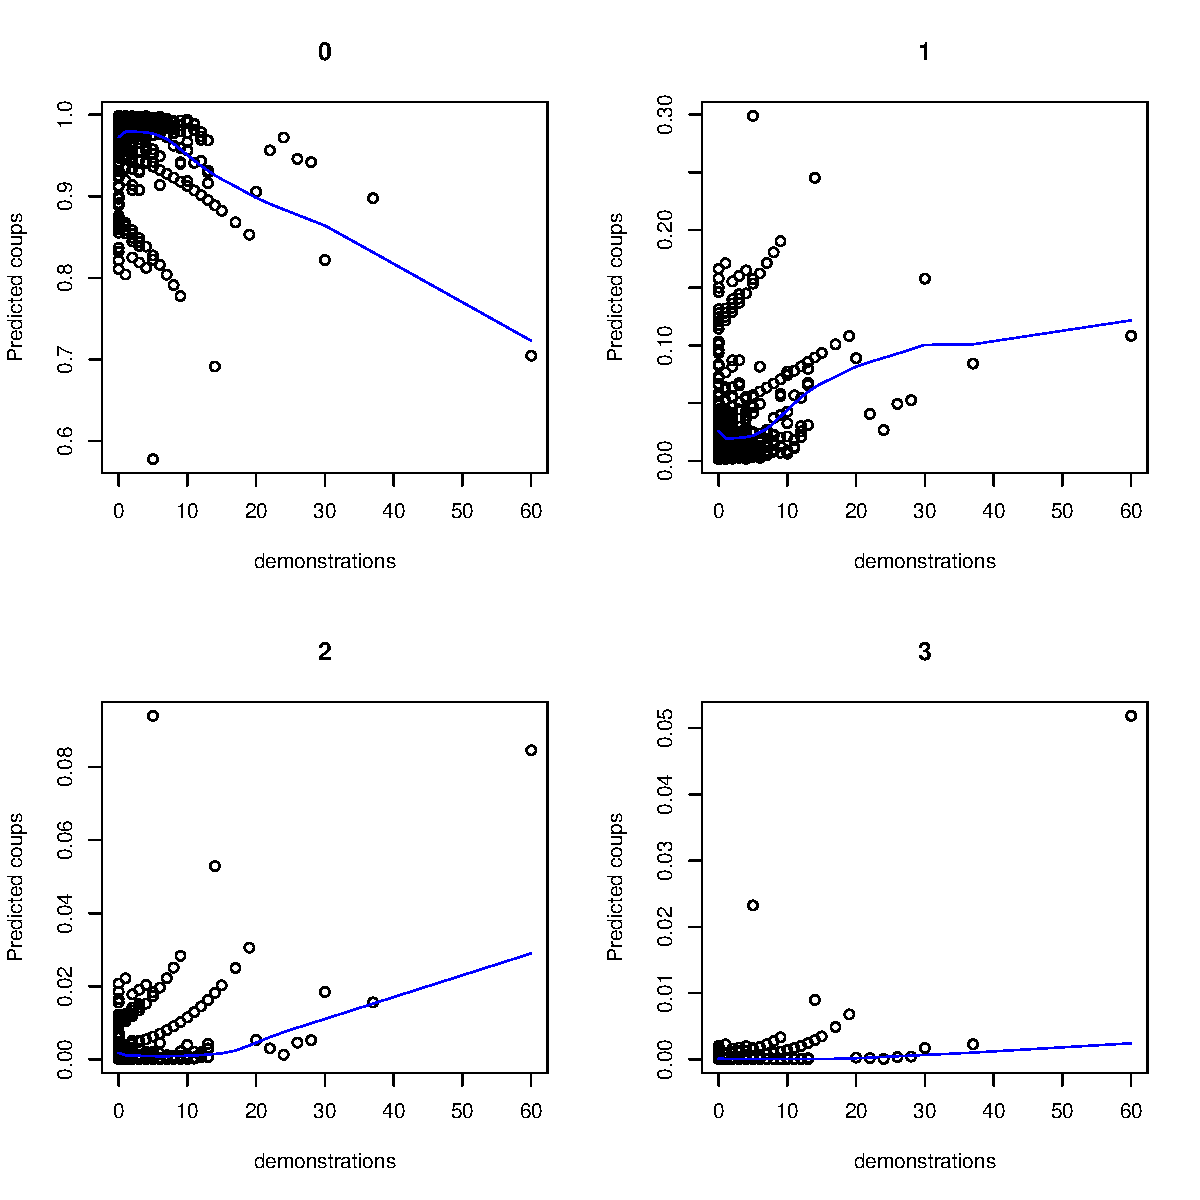
\includegraphics[width=\maxwidth]{figure/pp:plot-1} 

}




Ahora veamos si la especificaci\'on ZIP tiene un mejor \emph{fit} que la especificaci\'on ZINB. Para esto usaremos el Vuong test. Primero

\begin{knitrout}
\definecolor{shadecolor}{rgb}{0.969, 0.969, 0.969}\color{fgcolor}\begin{kframe}
\begin{alltt}
\hlkwd{p_load}\hlstd{(MASS)}
\hlkwd{vuong}\hlstd{(modelo.zip, modelo.zinb)}
\end{alltt}
\begin{verbatim}
## Vuong Non-Nested Hypothesis Test-Statistic: 
## (test-statistic is asymptotically distributed N(0,1) under the
##  null that the models are indistinguishible)
## -------------------------------------------------------------
##               Vuong z-statistic             H_A p-value
## Raw                  -0.3531275 model2 > model1   0.362
## AIC-corrected        -0.3531275 model2 > model1   0.362
## BIC-corrected        -0.3531275 model2 > model1   0.362
\end{verbatim}
\end{kframe}
\end{knitrout}

Considerando que la hip\'otesis nula es que \emph{the models are indistinguishible}, y que nuestro p-value no es significativo, no tenemos evidencia suficiente para determinar que la hipotesis alternativa (``the two models are {\bf NOT} indistinguishible'') se sostiene. Por lo tanto, los dos modelos son iguales (o ``indistinguishible'') y el segundo modelo (``ZINB'') {\bf NO} hace un mejor trabajo que el ``ZIP''.

\subsection{Rare-event Logistic Regression}

En esta secci\'on estimaremos un \texttt{relogit}. El paquete de \texttt{R} que usaremos se llama \texttt{Zelig}. 


Carguemos los datos:

\begin{knitrout}
\definecolor{shadecolor}{rgb}{0.969, 0.969, 0.969}\color{fgcolor}\begin{kframe}
\begin{alltt}
\hlkwd{install.packages}\hlstd{(}\hlstr{"https://cran.r-project.org/src/contrib/Archive/Zelig/Zelig_5.0-12.tar.gz"}\hlstd{,} \hlkwc{repos}\hlstd{=}\hlkwa{NULL}\hlstd{,} \hlkwc{type}\hlstd{=}\hlstr{"source"}\hlstd{)}
\hlkwd{library}\hlstd{(Zelig)}
\hlkwd{data}\hlstd{(mid)} \hlcom{# Militarized Interstate Disputes}
\hlstd{mid} \hlkwb{=} \hlkwd{na.omit}\hlstd{(mid)} \hlcom{# Omitir NAs}
\end{alltt}
\end{kframe}
\end{knitrout}

Hagamos un resumen,

\begin{knitrout}
\definecolor{shadecolor}{rgb}{0.969, 0.969, 0.969}\color{fgcolor}\begin{kframe}
\begin{alltt}
\hlkwd{summary}\hlstd{(mid)}
\end{alltt}
\begin{verbatim}
##     conflict          major            contig           power          
##  Min.   :0.0000   Min.   :0.0000   Min.   :0.0000   Min.   :0.0004201  
##  1st Qu.:0.0000   1st Qu.:0.0000   1st Qu.:0.0000   1st Qu.:0.0945675  
##  Median :0.0000   Median :0.0000   Median :0.0000   Median :0.3030594  
##  Mean   :0.3333   Mean   :0.1711   Mean   :0.2514   Mean   :0.3703210  
##  3rd Qu.:1.0000   3rd Qu.:0.0000   3rd Qu.:1.0000   3rd Qu.:0.6013527  
##  Max.   :1.0000   Max.   :1.0000   Max.   :1.0000   Max.   :0.9998207  
##      maxdem            mindem            years      
##  Min.   :-10.000   Min.   :-10.000   Min.   : 0.00  
##  1st Qu.: -5.000   1st Qu.: -9.000   1st Qu.: 3.00  
##  Median :  8.000   Median : -7.000   Median :11.00  
##  Mean   :  3.689   Mean   : -5.282   Mean   :13.97  
##  3rd Qu.: 10.000   3rd Qu.: -6.000   3rd Qu.:23.00  
##  Max.   : 10.000   Max.   : 10.000   Max.   :46.00
\end{verbatim}
\end{kframe}
\end{knitrout}

En esta aplicaci\'on pensaremos en la variable \texttt{conflict}: dummy para conflictos armados.

\begin{knitrout}
\definecolor{shadecolor}{rgb}{0.969, 0.969, 0.969}\color{fgcolor}\begin{kframe}
\begin{alltt}
\hlkwd{table}\hlstd{(mid}\hlopt{$}\hlstd{conflict)}
\end{alltt}
\begin{verbatim}
## 
##    0    1 
## 2084 1042
\end{verbatim}
\end{kframe}
\end{knitrout}


Estimemos un \texttt{relogit}.

\begin{knitrout}
\definecolor{shadecolor}{rgb}{0.969, 0.969, 0.969}\color{fgcolor}\begin{kframe}
\begin{alltt}
\hlstd{relogit.m} \hlkwb{<-} \hlkwd{zelig}\hlstd{(conflict} \hlopt{~} \hlstd{major} \hlopt{+} \hlstd{contig} \hlopt{+} \hlstd{power} \hlopt{+} \hlstd{maxdem} \hlopt{+} \hlstd{mindem} \hlopt{+} \hlstd{years,}
                \hlkwc{data} \hlstd{= mid,} \hlkwc{model} \hlstd{=} \hlstr{"relogit"}\hlstd{)}
\end{alltt}
\begin{verbatim}
## How to cite this model in Zelig:
##   Christine Choirat, James Honaker, Kosuke Imai, Gary King, and Olivia Lau. 2020.
##   relogit: Rare Events Logistic Regression for Dichotomous Dependent Variables
##   in Christine Choirat, James Honaker, Kosuke Imai, Gary King, and Olivia Lau,
##   "Zelig: Everyone's Statistical Software," http://zeligproject.org/
\end{verbatim}
\end{kframe}
\end{knitrout}




Ve\'amos el modelo,

\begin{knitrout}
\definecolor{shadecolor}{rgb}{0.969, 0.969, 0.969}\color{fgcolor}\begin{kframe}
\begin{alltt}
\hlkwd{summary}\hlstd{(relogit.m)}
\end{alltt}
\begin{verbatim}
## Model: 
## 
## Call:
## z5$zelig(formula = conflict ~ major + contig + power + maxdem + 
##     mindem + years, data = mid)
## 
## Deviance Residuals: 
##     Min       1Q   Median       3Q      Max  
## -3.0742  -0.4444  -0.2772   0.3295   3.1556  
## 
## Coefficients:
##              Estimate Std. Error z value             Pr(>|z|)
## (Intercept) -2.535496   0.179685 -14.111 < 0.0000000000000002
## major        2.432525   0.157561  15.439 < 0.0000000000000002
## contig       4.121869   0.157650  26.146 < 0.0000000000000002
## power        1.053351   0.217243   4.849          0.000001243
## maxdem       0.048164   0.010065   4.785          0.000001708
## mindem      -0.064825   0.012802  -5.064          0.000000411
## years       -0.063197   0.005705 -11.078 < 0.0000000000000002
## 
## (Dispersion parameter for binomial family taken to be 1)
## 
##     Null deviance: 3979.5  on 3125  degrees of freedom
## Residual deviance: 1868.5  on 3119  degrees of freedom
## AIC: 1882.5
## 
## Number of Fisher Scoring iterations: 6
## 
## Next step: Use 'setx' method
\end{verbatim}
\end{kframe}
\end{knitrout}


Usemos \emph{predicted probabilities}. Este enfoque de interpretaci\'on mezcla la tradici\'on Bayesiana y frecuentista. El estudiante interesado podr\'a referirse a \textcite{King2000}.

\begin{knitrout}
\definecolor{shadecolor}{rgb}{0.969, 0.969, 0.969}\color{fgcolor}\begin{kframe}
\begin{alltt}
\hlstd{x.high} \hlkwb{<-} \hlkwd{setx}\hlstd{(relogit.m,} \hlkwc{power} \hlstd{=} \hlkwd{quantile}\hlstd{(mid}\hlopt{$}\hlstd{power,} \hlkwc{prob} \hlstd{=} \hlnum{0.75}\hlstd{))}
\hlstd{x.low} \hlkwb{<-} \hlkwd{setx}\hlstd{(relogit.m,} \hlkwc{power} \hlstd{=} \hlkwd{quantile}\hlstd{(mid}\hlopt{$}\hlstd{power,} \hlkwc{prob} \hlstd{=} \hlnum{0.25}\hlstd{))}
\hlstd{s.out2} \hlkwb{<-} \hlkwd{sim}\hlstd{(relogit.m,} \hlkwc{x} \hlstd{= x.high,} \hlkwc{x1} \hlstd{= x.low)}
\hlkwd{par}\hlstd{(}\hlkwc{mar}\hlstd{=}\hlkwd{c}\hlstd{(}\hlnum{1}\hlstd{,}\hlnum{1}\hlstd{,}\hlnum{1}\hlstd{,}\hlnum{1}\hlstd{))}
\hlkwd{plot}\hlstd{(s.out2)}
\end{alltt}
\end{kframe}

{\centering 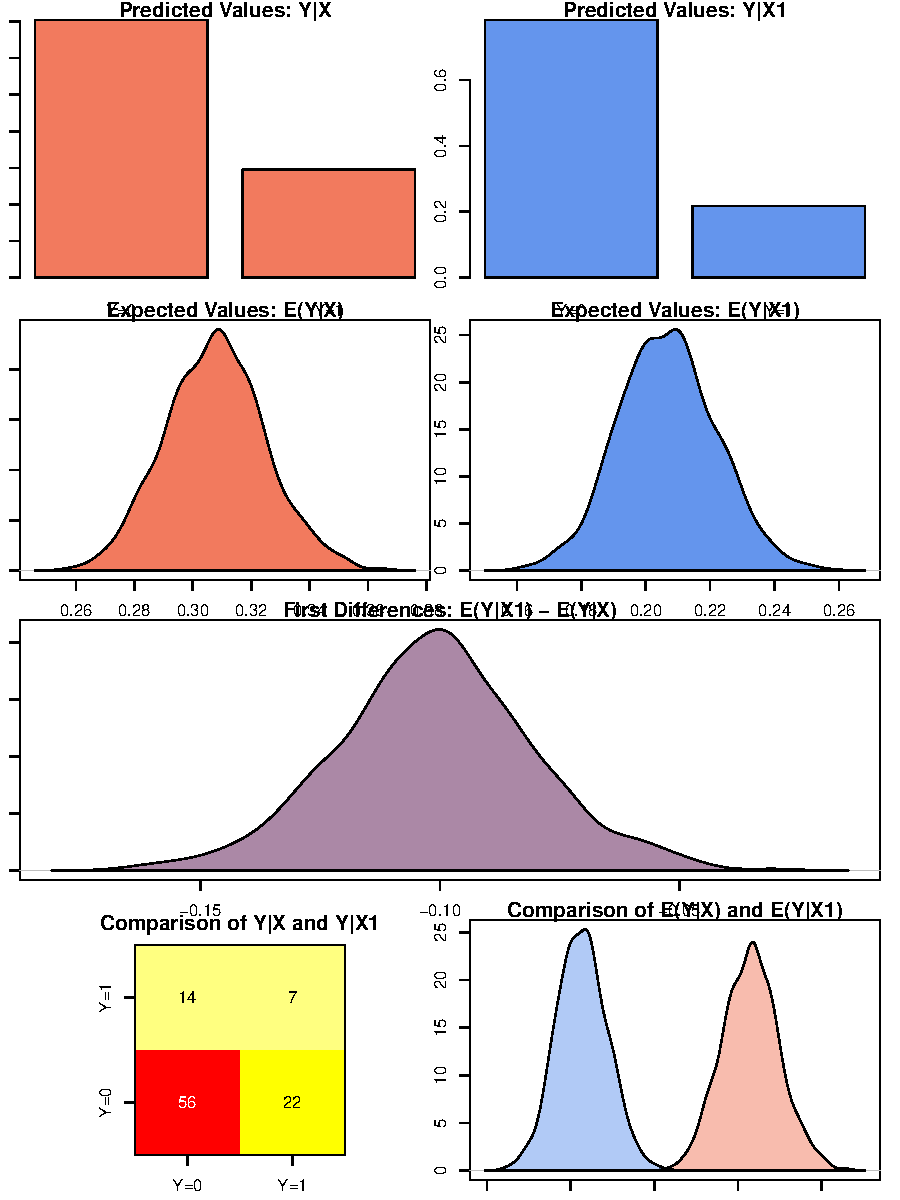
\includegraphics[width=\maxwidth]{figure/zelig:plot-1} 

}



\end{knitrout}





\begin{knitrout}
\definecolor{shadecolor}{rgb}{0.969, 0.969, 0.969}\color{fgcolor}\begin{kframe}
\begin{alltt}
\hlstd{knitr}\hlopt{::}\hlkwd{purl}\hlstd{(}\hlstr{'ZIP_ZINB_RELOGIT.Rnw'}\hlstd{)}
\end{alltt}


{\ttfamily\noindent\bfseries\color{errorcolor}{\#\# Error in parse\_block(g[-1], g[1], params.src, markdown\_mode): Duplicate chunk label 'setup', which has been used for the chunk:\\\#\# if (!require("{}pacman"{})) install.packages("{}pacman"{}); library(pacman)\\\#\# p\_load(knitr)\\\#\# set.seed(2020)\\\#\# options(scipen=9999999)}}\begin{alltt}
\hlkwd{Stangle}\hlstd{(}\hlstr{'ZIP_ZINB_RELOGIT.Rnw'}\hlstd{)}
\end{alltt}
\begin{verbatim}
## Writing to file ZIP_ZINB_RELOGIT.R
\end{verbatim}


{\ttfamily\noindent\bfseries\color{errorcolor}{\#\# Error in match.arg(options\$results, c("{}verbatim"{}, "{}tex"{}, "{}hide"{})): 'arg' should be one of "{}verbatim"{}, "{}tex"{}, "{}hide"{}}}\end{kframe}
\end{knitrout}


\newpage
\paragraph{}
\paragraph{}
\pagenumbering{Roman}
\setcounter{page}{1}
\printbibliography



\end{document}

